
In Section~\ref{sec: introduction} we gave an outline of the algorithm
proposed by Dinh~\etal~\cite{dinh2014network} for computing mixing graphs
with minimum waste. The algorithm relies on the assumption that an
optimum mixing graph (that is, the graph that minimizes waste)
for a target set with maximum precision $d$ has depth at most $d$.
This seems indeed intuitive --- yet we show that this assumption is not valid,
by constructing a target set $T$ with maximum precision $d$ that requires
depth at least $2d-1$ to be produced by a mixing graph (without waste).

Our target set is
$T = \braced{ \, 2^{-d} \,,\, ((d-1)2^d+1): (1-2^{-d})\, }$,
that is, $T$ has one droplet with concentration $2^{-d}$ and $(d-1)2^d+1$ droplets with
concentration $1-2^{-d}$. 

We first observe that there is a mixing graph of depth $2d-1$ that produces $T$ without waste.
(See Figure~\ref{fig: dinh counterexample}.)
This graph first mixes $0$ and $1$, producing two droplets $\half$.
One droplet $\half$ is mixed $d-1$ times with $0$. This creates a path with
$d-1$ mixers that produce
droplets $2^{-2}, 2^{-3},...,2^{-d}$, plus one more droplet $2^{-d}$ that is sent to the output.
The other droplet $\half$, symmetrically, is mixed repeatedly with $1$,
producing
droplets $1-2^{-2}, 1-2^{-3},...,1-2^{-d}$, plus one more droplet $1-2^{-d}$ that is sent to the output.
For $a = 2,...,d$, we can then mix each droplet 
$2^{-a}$ with $1-2^{-a}$, which produces $2(d-1)$ droplets $\half$.
Each droplet $\half$ can be then mixed repeatedly ($d-1$ times) with $1$'s,
creating a tree-like subgraph of depth $d-1$ that produces
$2^{d-1}$ droplets $1-2^{-d}$. Thus, overall, we produce
one droplet $2^{-d}$ and $(d-1)2^d+1$ droplets $1-2^{-d}$, which is exactly $T$.
The depth of this graph is $2d-1$.

%%%%%%
	
\begin{figure}[ht]
	\begin{center}
		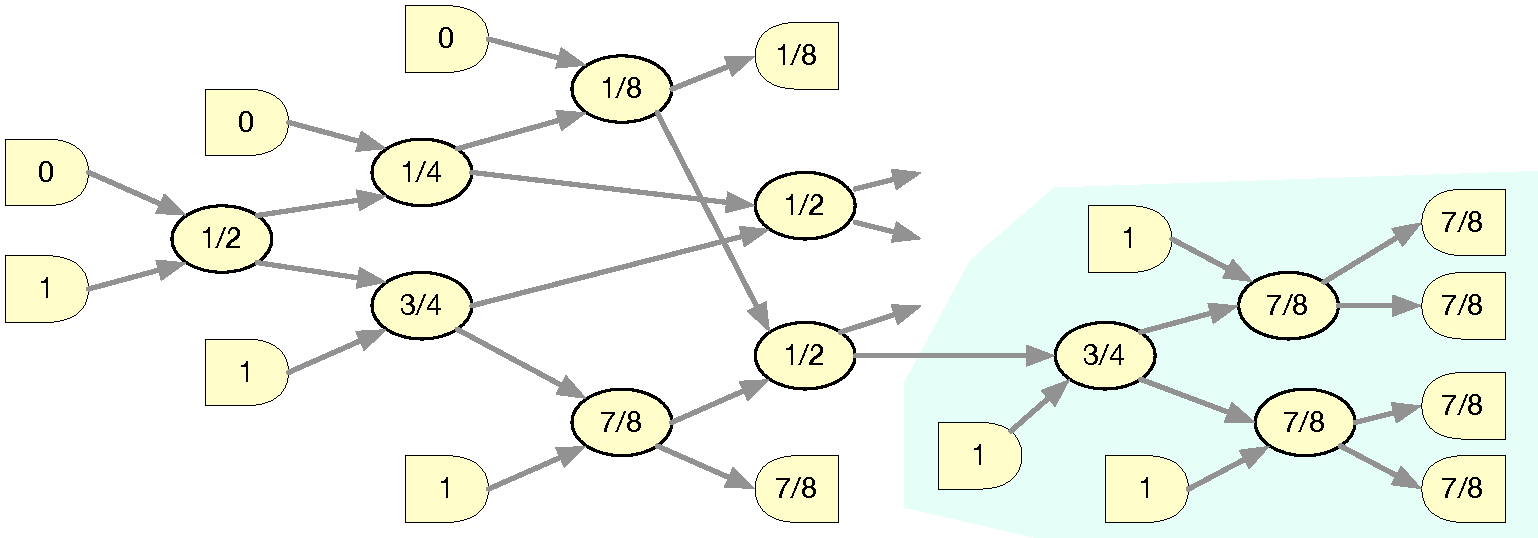
\includegraphics[width = 5.2in]{dinh_counterexample.pdf}
		\caption{A mixing graph of depth $d=5$ that
		 	produces $T = \braced{ \, \oneeighth \, ,\, 17 : \seveneighths \,}$.
			Only one subgraph converting $\half$ into droplets $\seveneighths$ is shown (on shaded background).}
		\label{fig: dinh counterexample}
	\end{center}
\end{figure}


Next, we claim that producing $T$ without any waste requires depth $2d-1$.
The argument is as follows. Consider a micro-mixer that produces 
droplet $2^{-d}$ of $T$. This mixer actually produces \emph{two} droplets $2^{-d}$
and is at depth at least $d$, because it takes $d$ steps to dilute $1$ to
concentration $2^{-d}$. The fluid in the second droplet $2^{-d}$ (the one not in $T$) 
produced by this mixer
must also end up in some droplets of $T$ and its concentration will increase
to $1-2^{-d}$. The \emph{buffer concentration} in this droplet is $1-2^{-d}$ and it
takes at least $d-1$ steps to reduce it to $2^{-d}$, in order to
obtain a droplet with reactant concentration $1-2^{-d}$. We can therefore
conclude that the depth of any mixing graph for $T$ is at least $2d-1$.



	